% vim: set fenc=utf-8 ft=latex
% !Mode:: "TeX:UTF-8"
% !TEX encoding = UTF-8 Unicode 
% -*- mode: latex -*-
% -*- coding: UTF-8 -*-
% kate: encoding utf-8;
%
% IMPORTANT Note: This file is UTF-8 encoded! 
%                 You should see some umlauts here: ÄÖÜäöü 

\documentclass[french,12pt,a4paper,twoside,openright,titlepage]{report}
\usepackage{algorithm}
\usepackage{algorithmic}
\usepackage[utf8]{inputenc}
\usepackage{fancyhdr}
\usepackage{amsmath}
\usepackage{amssymb}
\usepackage{babel}
\usepackage{amsfonts}
\usepackage{graphicx}
%\usepackage{here}
\usepackage{hyperref}
\usepackage{ifthen}
\usepackage{xcomment}
\usepackage{array}
\usepackage{rotating}
\usepackage{listings}
%\usepackage{enumitem}
\textwidth17cm
\textheight25cm
%\oddsidemargin-1cm
%\parskip0.2pt
\voffset-2cm
\hoffset-1cm
\headsep0.5cm
\topmargin0.5cm
\oddsidemargin0.5cm
\evensidemargin0.5cm

\makeatletter
\@addtoreset{section}{part}
\makeatother
\newlength{\mylength}
\newcounter{exo}\stepcounter{exo}
\newcounter{step}\stepcounter{step}
\newcommand\exercice{
\subsubsection*{Exercice \theexo\stepcounter{exo}}
%{\bf Exercice \theexo\stepcounter{exo}\\}
}
\newcommand\etape[1]{
\subsection*{Etape \thestep \stepcounter{step} : {#1}}
}
 
\RequirePackage{layout,color}

\definecolor{gray50}{gray}{.5}
\definecolor{gray40}{gray}{.6}
\definecolor{gray30}{gray}{.7}
\definecolor{gray20}{gray}{.8}
\definecolor{gray10}{gray}{.9}
\definecolor{gray05}{gray}{.95}

\newsavebox{\laboiboite}
\newlength{\longdelaboiboite}
\newlength{\deptdelaboiboite}
\newlength{\hautdelaboiboite}
\newcolumntype{R}{>{\begin{lrbox}{\laboiboite} 
$\displaystyle }r<{$\end{lrbox}%
    \settowidth{\longdelaboiboite}{\usebox{\laboiboite}}%
    \settoheight{\hautdelaboiboite}{\usebox{\laboiboite}}%
    \settodepth{\deptdelaboiboite}{\usebox{\laboiboite}}%
    \addtolength{\hautdelaboiboite}{\deptdelaboiboite}%
    \addtolength{\hautdelaboiboite}{2ex}%
    \parbox[c][\hautdelaboiboite][c]{0cm}{} \makebox[\width]
{\usebox{\laboiboite}}}}
\newcolumntype{C}{>{\begin{lrbox}{\laboiboite} 
$\displaystyle }c<{$\end{lrbox}%
    \settowidth{\longdelaboiboite}{\usebox{\laboiboite}}%
    \settoheight{\hautdelaboiboite}{\usebox{\laboiboite}}%
    \settodepth{\deptdelaboiboite}{\usebox{\laboiboite}}%
    \addtolength{\hautdelaboiboite}{\deptdelaboiboite}%
    \addtolength{\hautdelaboiboite}{2ex}%
    \parbox[c][\hautdelaboiboite][c]{0cm}{} \makebox[\width]
{\usebox{\laboiboite}}}}
\newcolumntype{L}{>{\begin{lrbox}{\laboiboite} 
$\displaystyle }l<{$\end{lrbox}%
    \settowidth{\longdelaboiboite}{\usebox{\laboiboite}}%
    \settoheight{\hautdelaboiboite}{\usebox{\laboiboite}}%
    \settodepth{\deptdelaboiboite}{\usebox{\laboiboite}}%
    \addtolength{\hautdelaboiboite}{\deptdelaboiboite}%
    \addtolength{\hautdelaboiboite}{2ex}%
    \parbox[c][\hautdelaboiboite][c]{0cm}{} \makebox[\width]
{\usebox{\laboiboite}}}}

\newcolumntype{S}{>{\begin{lrbox}{\laboiboite}}r<{\end{lrbox}%
    \mbox{\usebox{\laboiboite}}}}
\newcolumntype{D}{>{\begin{lrbox}{\laboiboite}}c<{\end{lrbox}%
    \mbox{\usebox{\laboiboite}}}}
\newcolumntype{M}{>{\begin{lrbox}{\laboiboite}}l<{\end{lrbox}%
    \mbox{\usebox{\laboiboite}}}}
\newlength\Linewidth
\def\findlength{\setlength\Linewidth\linewidth
\addtolength\Linewidth{-4\fboxrule}
\addtolength\Linewidth{-3\fboxsep}
}
\newenvironment{examplebox}{\par\begingroup%
   \setlength{\fboxsep}{5pt}\findlength%
   \setbox0=\vbox\bgroup\noindent%
   \hsize=\Linewidth%
   \begin{minipage}{\Linewidth}\small}%
    {\end{minipage}\egroup%
    \vspace{6pt}%
    \noindent\textcolor{gray20}{\fboxsep2.5pt\fbox%
     {\fboxsep5pt\colorbox{gray05}{\normalcolor\box0}}}%
    \endgroup\par\addvspace{6pt minus 3pt}\noindent%
    \normalcolor\ignorespacesafterend}
\let\Examplebox\examplebox
\let\endExamplebox\endexamplebox

\lstset{ %
 frame=single,	       
 language=C,
}
\usepackage{color}
\lstset{
	language=C, 
	breaklines=true, 
	tabsize=2, 
	keywordstyle=\color{blue}, 
	commentstyle=\color{gray50}, 
	stringstyle=\color{red}, 
	basicstyle=\tt,
	morekeywords={True,False},
	frame=single
}






\makeatletter
\renewcommand{\thesection}{\@arabic\c@section}
\makeatother

%%%%%%%%%%%%%%%%%%%%%%%%%%%%%%%%%%%%%%%%%%%%%%%%%%%%%%%%%%%%%%
%%%%%%%%%%%%%%%%%%%%%%%%%%%%%%%%%%%%%%%%%%%%%%%%%%%%%%%%%%%%%%
%%%%%%%%%%%%%%%%%%%%%%%%%%%%%%%%%%%%%%%%%%%%%%%%%%%%%%%%%%%%%%
\newboolean{sol}
%\setboolean{sol}{true}
\setboolean{sol}{false}
%%%%%%%%%%%%%%%%%%%%%%%%%%%%%%%%%%%%%%%%%%%%%%%%%%%%%%%%%%%%%%
%%%%%%%%%%%%%%%%%%%%%%%%%%%%%%%%%%%%%%%%%%%%%%%%%%%%%%%%%%%%%%
%%%%%%%%%%%%%%%%%%%%%%%%%%%%%%%%%%%%%%%%%%%%%%%%%%%%%%%%%%%%%M
\ifthenelse{\boolean{sol}}
{
\newenvironment{solution}
{
\begin{examplebox}
\begin{center}
\begin{tabular}{m{0.5cm}|m{15cm}|}\cline{2-2}
%\begin{turn}{90}{Solution}\end{turn}&
\rotatebox{90}{Solution}&
\begin{minipage}[H]{\linewidth}
\vspace{0.2cm}
}
{
\vspace{0.2cm}
\end{minipage}
\\\cline{2-2}
\end{tabular}
\end{center}
\end{examplebox}
}
}
{
\newxcomment[]{solution}
}


\newcommand{\ROBorMAIN}{ROB}%set to MAIN or to ROB
\newcommand{\ROBMAIN}[2]{\ifthenelse{\equal{\ROBorMAIN}{ROB}}{#1}{#2}}




\begin{document}

\lhead[ROB3/MAIN3]{ROB3/MAIN3}
\chead[]{}
\rhead[Informatique général]{}
 
\ifthenelse{\boolean{sol}}
{
\lfoot[Polytech'Paris-UPMC 2016-2016 (version enseignants)]{Polytech'Paris-UPMC 2016-2017 (version enseignants)}

}
{
\lfoot[Polytech'Paris-UPMC 2016-2017 (version \'etudiants)]{Polytech'Paris-UPMC 2016-2017 (version \'etudiants)}
}

\cfoot[]{}
\rfoot[\thepage]{\thepage}




\pagestyle{fancyplain}
%%%%%%%%%%%%

 %\addcontentsline{toc}{chapter}{S\'erie 1 : Conception d'algorithmes}
 %\chapter{Conception d'algorithmes}
 %\addcontentsline{toc}{chapter}{S\'erie 1 : Conception d'algorithmes}

\chapter*{Mini-Projet : Labyrinthe}

L'objectif du projet est de programmer un jeu de Labyrinthe de façon à ce que votre programme puisse jouer une partie contre les programmes des autres étudiants.

\section{Organisation générale du projet}

Ce projet se déroulera en binôme (ou trinôme si nombre impair). Le choix des binômes est libre. La soutenance du projet aura lieu en deux temps : 
\begin{itemize}
\item une soutenance orale de 15 minutes (avec supports Power-Point (ou Beamer/\LaTeX) le \textbf{17 Janvier 2016} ;
\item un tournoi de Labyrinthe entre les binômes. Le gagnant du tournoi aura l'honneur de rencontrer un programme réalisé par un enseignant et invaincu (par définition) jusqu'à aujourd'hui. Les modalités détaillées de la soutenance seront précisées mi-décembre. Le tournoi sera commun entre les spécialités ROB et MAIN.
\end{itemize}

\subsection{Déroulement du projet}
Le projet se déroulera à partir du 29 Novembre. Vous bénéficierez de 3 séances de TP encadrées pour la réalisation de ce projet. L'encadrant de TP aura le rôle de chef de projet. C'est donc lui qui vous conseillera et vous guidera pour les étapes importantes, et c'est aussi lui qui validera la réalisation de chacune des étapes du projet.

\subsection{Assistance}
À tout moment il vous est possible de poser une question sur la plateforme Piazza dédiée à l'adresse suivante :
\begin{center}
%\url{http://piazza.com/upmc.fr/winter2016/pipopipette/home}
\url{https://piazza.com/upmc.fr/fall2016/laby/home}
\end{center}
Vous allez très rapidement recevoir un email pour vous y inscrire.\\
Cette plateforme permet à chacun de poser des questions sur un forum dédié au projet. Cela vous permettra de poser vos questions en dehors des séances de TP encadrées et d'obtenir des conseils ou de l'aide. Vous pouvez aussi utiliser ce forum entre vous pour vous aider (vous aider et non pas sous-traiter votre code!). N'hésitez pas à l'utiliser !


\subsection{Évaluation}
Le projet sera évalué sur les critères suivants : 
\begin{itemize}
\item L'avancement du projet au fur et à mesure (validation des étapes);
\item La soutenance orale;
\item La qualité du programme final (bugs, fonctionnalités codées, etc.);
\item La place au tournoi de Labyrinthe.
\end{itemize}

\section{Règles du jeu}
\subsection{Le but du jeu}
Vous êtes deux adversaires dans un labyrinthe. Un trésor (et un seul)
est présent au milieu du labyrinthe.

\textbf{L'objectif est d'être le premier à récupérer le trésor.}

\subsection{Données d'une partie}
\begin{figure}[h]
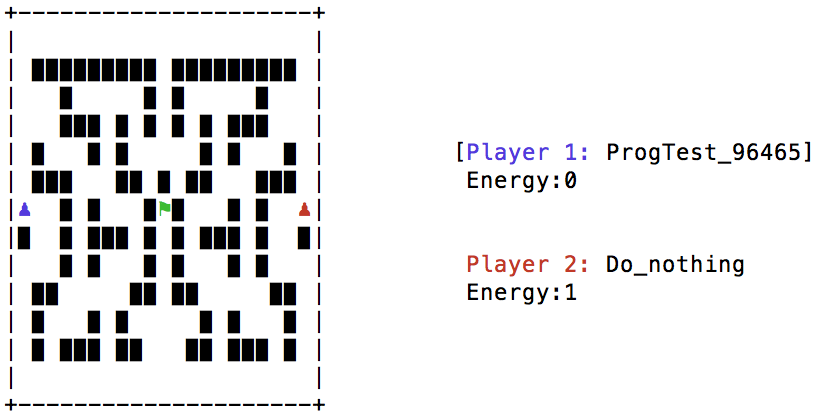
\includegraphics[width=\textwidth]{./laby-init.png}
\caption{\label{fig:init} Exemple d'un labyrinthe en début de partie. La case de coordonnées (0,0) est située en haut à gauche.}
\end{figure}
En début de partie le serveur de jeu vous envoie les informations suivantes :
\begin{itemize}
\item La taille du labyrinthe en hauteur $H$ et longueur $L$ via la fonction \verb|waitForLabyrinth| (cf~\ref{sec:wait}). La taille
est aléatoire et telle que $L$ et $H$ soient impairs, $13\leq L\leq 17$ et $9\leq H\leq 15$ ;
\item Le nom du labyrinthe ;
\item Les données du labyrinthe : Les positions des murs (infranchissables) et des espaces libres. Sur la figure~\ref{fig:init}, les murs sont indiqués par des carrés noirs. Pour plus de détail, voir la fonction \verb|getLabyrinth| (cf~\ref{sec:getlab}) ;
\item L'indication du joueur qui commence.
\end{itemize}

Ensuite, vous pouvez construire le labyrinthe initial sachant que :
\begin{itemize}
\item Le joueur qui commence est situé sur la case de coordonnées $x=0$ et $y=H/2$ (division entière);
\item L'autre joueur est situé sur la case de coordonnées $x=L-1$ et $y=H/2$ (division entière);
\item Le trésor est situé sur la case de coordonnées $x=L/2$ et $y=H/2$ (division entière);
\item Le joueur qui commence a un niveau initial d'énergie de $0$, l'autre joueur a un niveau initial d'énergie de $1$.
\end{itemize}
\textbf{Notez que les coordonnées $x=0$ et $y=0$ correspondent à la case située en haut à gauche.}

Ensuite, à chaque tour de jeu, vous pouvez soit effectuer un déplacement classique de votre joueur, soit (sous certaines conditions) effectuer une rotation du labyrinthe.

\subsection{Déplacement classique d'un joueur}
\begin{figure}
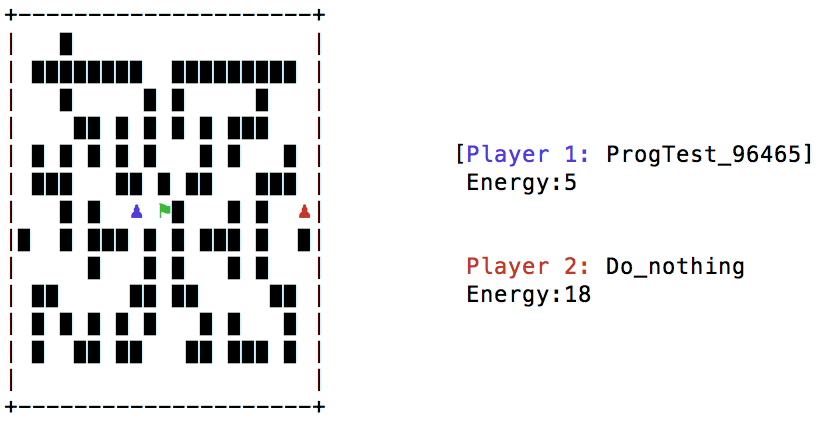
\includegraphics[width=\textwidth]{laby-m2.png}\\
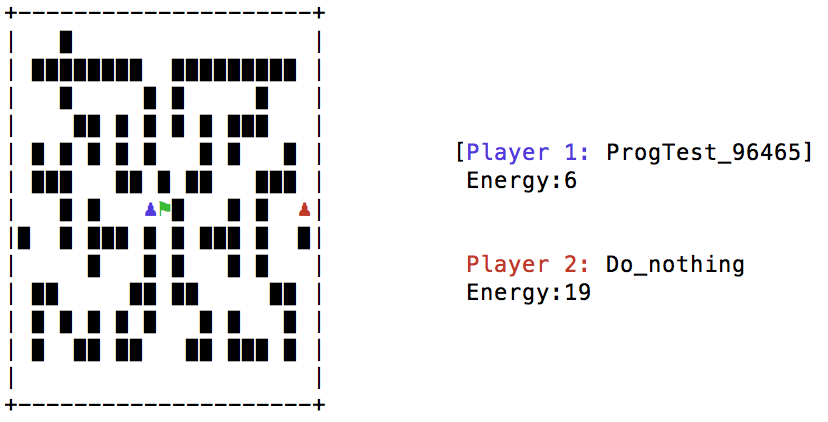
\includegraphics[width=\textwidth]{laby-m1.png}
\caption{\label{fig:move}Déplacement du joueur 1 vers la droite}
\end{figure}

À chaque tour vous pouvez vous déplacer d'une case vers une case libre (c'est-à-dire sans mur) vers 
le haut, le bas, la gauche ou la droite. Vous pouvez aussi rester sur place. La figure~\ref{fig:move} montre
un exemple de déplacement.
\begin{itemize}
\item À chaque fois que vous faites un déplacement de ce type, vous gagnez une unité d'énergie ;
\item Vous ne pouvez pas vous déplacer sur un mur, par contre, vous pouvez vous déplacer sur votre adversaire,
ou sur le trésor (dans ce cas vous le récupérez);
\item Le labyrinthe est circulaire (et même toroïde !), un joueur sortant à gauche se retrouve tout à droite
et un joueur sortant en haut se retrouve en bas.
\end{itemize}

\subsection{Rotation du labyrinthe}
\begin{figure}
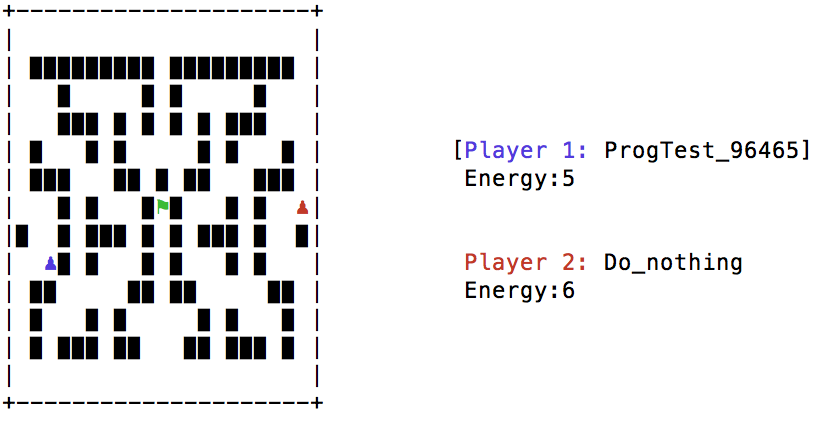
\includegraphics[width=\textwidth]{laby-r1.png}\\
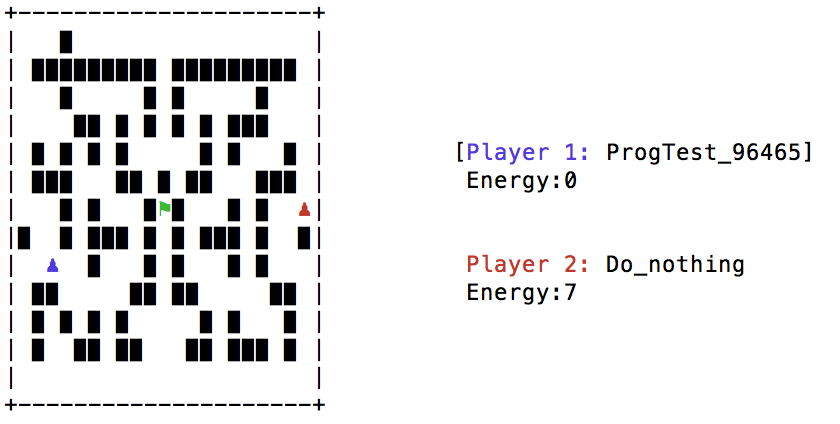
\includegraphics[width=\textwidth]{laby-r2.png}
\caption{\label{fig:rot} Rotation de la colonne 3 vers le haut}
\end{figure}

À chaque tour vous pouvez dépenser 5 unités d'énergie pour décaler une ligne
(ou une colonne) entière du labyrinthe d'une case vers la gauche ou vers la droite
 (haut/bas pour la colonne). La figure~\ref{fig:rot} présente un exemple de rotation.
 
 \begin{itemize}
 \item La rotation est circulaire : la case sortante d'un côté entre de l'autre ;
\item Les joueurs ou le trésor se déplacent avec la rotation du labyrinthe.
 \end{itemize}

\subsection{Conditions de fin de partie}
~\label{sec:endgame}
Conditions de victoire :

\begin{itemize}
\item Vous atteignez le trésor en premier;
\item Votre adversaire perd avant.
\end{itemize}

Conditions de défaite :
\begin{itemize}
\item Votre adversaire atteint le trésor avant vous;
\item Vous faites un coup illégal (ex : déplacement dans un mur);
\item Vous tentez de faire une rotation, mais n'avez pas assez d'énergie;
\item Vous ne respectez pas le séquencement du programme (cf section~\ref{sec:sequences});
\item Vous mettez trop de temps à jouer (max. 10 secondes).
\end{itemize}


\section{Structure du programme}
Votre programme Labyrinthe devra se connecter à un serveur de jeu qui a deux rôles :
\begin{enumerate}
\item Mettre en relation des programmes afin de les faire jouer entre eux;
\item Vérifier la validité des coups joués et déclarer le joueur gagnant.
\end{enumerate}

\subsection{Fichiers fournis}
\label{sec:fourni}
Tous les fichiers qui vous sont fournis dans le cadre de ce projet sont disponible sur le serveur de Polytech
aux emplacements \verb|/home/sasl/encad/brajard/projet/CGS_distrib| et \verb|/home/sasl/encad/brajard/projet/CGS_lib|.
Il vous est conseillé de :
\begin{itemize}
\item Copier sur votre compte les fichiers \verb|template.c| et \verb|makefile| fournis que vous pourrez modifier (tout le contenu du répertoire \verb|CGS_distrib|)\\
Par exemple, si vous êtes dans le répertoire dans lequel vous souhaitez réaliser votre projet, il suffit de faire :\\
\verb|cp /home/sasl/encad/brajard/projet/CGS_distrib/* .|
(n'oubliez pas le \verb|.| à la fin);
\item Ne pas changer les chemins vers les \textit{header} et \textit{bibliothèques}  indiquées dans le \verb|makefile| (ne pas copier le contenu du sous-répertoire \verb|CGS_lib| car il pourra potentiellement être mis à jour si nécessaire). Attention les bibliothèques ont été compilées sur les machine de polytech et ne fonctionnent donc qu'à Polytech (ou sur une machine équivalente).
\end{itemize}

On donne ci-après la structure générale de votre programme. Les fonctions appelées et les types utilisés sont détaillés
dans la section~\ref{sec:api}.  Les modèles de structure et les prototypes des fonctions sont décrits dans le fichier 
\verb|CGS_lib/include/labyrinthAPI.h|\\
Voici les différentes étapes que devra respecter votre programme pour interagir avec le serveur.

\subsection{Étapes à respecter dans votre programme}
\label{sec:sequences}
Ces étapes sont en grande partie (mais pas complètement) codées dans le fichier \verb|template.c| qui vous est fourni en début de projet (voir section~\ref{sec:fourni})
\begin{enumerate}
\item Se connecter au serveur en appelant la fonction \verb|connectToServer|;
\item Demander un Labyrinthe en appelant la fonction \verb|waitForLabyrinth| :
\begin{itemize}
\item Pour jouer contre un joueur par défaut toujours disponible, le spécifier avec le paramètre "training"

Ex: \texttt{training="DO\_NOTHING\_GAME timeout=n"} (en spécifiant une valeur pour \verb|n| (cf~\ref{sec:default}). D'autres adversaires par défaut peuvent être spécifiés. 

\item Pour joueur contre un autre programme, vous devez laisser l'option \texttt{training} vide (\verb|""|). Vous devez alors vous rendre sur la page web du serveur via un navigateur (ex : \url{http://pc4021.polytech.upmc.fr:8088} pour un serveur tournant sur le pc4021) et créer une rencontre entre vous et un autre joueur. Attention la page web n'est accessible que depuis une machine du réseau Poytech'.
\end{itemize}
\item Récupérer les données du labyrinthe en appelant la fonction \verb|getLabyrinth|;
\item Répéter les actions suivantes :
\begin{itemize}
\item Si c'est à vous de jouer : envoyer votre coup en appelant la fonction \verb|sendMove|, vous récupérez le code \verb|ret|.
\item Si c'est à l'adversaire de jouer : récupérer le coup joué par l'adversaire en appelant la fonction \verb|getMove|, vous récupérez également le code \verb|ret|.
\item En fonction de \verb|ret| :
\begin{itemize}
\item \verb|ret==MOVE_OK| : vous pouvez continuer à jouer;
\item \verb|ret==MOVE_LOSE| : le joueur qui vient de jouer à perdu;
\item \verb|ret==MOVE_WIN| : le joueur qui vient de jouer à gagné.
\end{itemize}
\end{itemize}
\item Fermer la connexion au serveur en appelant la fonction \verb|closeConnection|.
\end{enumerate}
De plus, à tout moment, vous pouvez demander l'affichage du jeu à l'écran en appelant la fonction \verb|printLabyrinth|.

\subsection{Les joueurs par défaut}
\label{sec:default}
Lors de l'appel de la fonction \verb|waitForLabyrinth|, il est possible de demander un joueur par défaut  ("training player").
Vous pourrez alors tester votre programme sans qu'un autre joueur ne se connecte sur le serveur.
Pour cela, il faut spécifier dans une chaîne de caractère \verb|training|  le nom de ce joueur par défaut, ainsi que les paramètres. Pour l'instant, deux joueurs par défaut sont disponibles : 
\begin{itemize}
\item \textbf{DO\_NOTHING} : Ce joueur ne fait aucun mouvement.

Exemple : \verb|training = "DO_NOTHING timeout=10"| pour le joueur DO\_NOTHING avec une limite de temps pour jouer (voir conditions de défaites~\ref{sec:endgame}) de 10 sec (Ce temps peut être changé).

\item \textbf{PLAY\_RANDOM} : Ce joueur joue aléatoirement, mais tous ses coups sont valides.

Exemple : \verb|training = "PLAY_RANDOM timeout=60 rotation=True"| pour jouer avec 60 s de limite de temps et la possibilité pour le joueur PLAY\_RANDOM de faire les rotations de lignes et colonnes dans le labyrinthe (mettre l'option à \verb|False| si on veut que PLAY\_RANDOM ne fasse que des déplacements classiques.)

\item \textbf{...} : D'autres joueurs par défaut viendront s'ajouter en cours de projet.

\end{itemize}

\section{\label{sec:api}API}


\subsection{Les structures à utiliser}

\subsubsection{La structure \texttt{t\_move}}
Cette structure décrit un coup joué par vous ou par votre adversaire, elle est utilisée dans les fonctions  \verb|sendMove| et \verb|getMove| :
\lstinputlisting[language=C, firstline=38, lastline=50]{../API/labyrinthAPI.h}
Par exemple :
\begin{itemize}
\item Une variable \verb|m| décrivant le déplacement d'une case vers la droite a pour valeurs

\verb|m.type = MOVE_RIGHT| et \verb|m.value = -1| (valeur non utilisée).
\item Une variable \verb|m| décrivant une rotation de la colonne 3 vers le haut a pour valeurs

\verb|m.type = ROTATE_COLUMN_UP| et  \verb|m.value = 3|. On rappelle ici que la première colonne
(et la première ligne) est numérotée 0.
\end{itemize}

\subsubsection{La structure \texttt{t\_return\_code}}
Cette structure décrit le code retour des fonctions \verb|sendMove| et \verb|getMove|. Elle permet de décrire si un coup qui vient d'être joué
est correct (\verb|MOVE_OK|), gagnant (\verb|MOVE_WIN|) ou perdant (\verb|MOVE_LOSE|). Cette valeur doit être testée
dans votre programme pour savoir si vous devez rejouer ou si la partie est terminée.

%\subsubsection{L'énumération \texttt{t\_gameType}}
%Cette énumération donne les choix de jeux possible (jouer seul ou contre un autre programme)
%Pour le moment seuls deux types de jeux sont prévus :
%\begin{itemize}
%\item \verb|DO_NOTHING_GAME| : pour jouer seul contre un adversaire qui ne fait rien.
%\item \verb|REGULAR_GAME| : pour jouer contre un autre programme
%\end{itemize}
%Dans le futur, d'autres types de jeu seront mis à disposition pour jouer seul.
%\lstinputlisting[language=C, firstline=53, lastline=62]{../API/labyrinthAPI.h}


\subsection{Fonctions fournies}
 
\subsubsection{\texttt{connectToServer}}
Permet de se connecter au serveur (à faire une seule fois, en début de programme).
\lstinputlisting[language=C, firstline=53, lastline=66]{../API/labyrinthAPI.h}
Le numéro de port et le nom du serveur vous seront donnés lors de la première séance.



\subsubsection{\texttt{closeConnection}}
Permet de se déconnecter du serveur (à la fin du programme).
\lstinputlisting[language=C, firstline=70, lastline=77]{../API/labyrinthAPI.h}


\subsubsection{\texttt{waitForLabyrinth}}
Permet d'attendre une partie Labyrinth, et de récupérer son nom et sa taille. Permet aussi de spécifier si on veut jouer contre un joueur d'entraînement.
\label{sec:wait}
\lstinputlisting[language=C, firstline=79, lastline=107]{../API/labyrinthAPI.h}
Les arguments \texttt{labyrinthName}, \texttt{sizeX} et \texttt{sizeY} sont passés via des pointeurs et leurs valeurs
seront donc données en sortie de fonction.


\subsubsection{\texttt{getLabyrinth}}
Permet de récupérer les données initiales du labyrinthe.
\label{sec:getlab}
\lstinputlisting[language=C, firstline=108, lastline=119]{../API/labyrinthAPI.h}
L'argument \texttt{lab} est passé via un pointeur et 
la valeur sera donc donnée en sortie de fonction. Le tableau \texttt{lab} rempli par cette
fonction est un tableau à 1 dimension de taille $L\times H$ qui contient des entiers (sur 8 bits). Les cases valent $0$ pour les cases libres et $1$ pour les murs. Il est rempli dans le sens des lignes, c'est-à-dire que les $L$
premières valeurs correspondent aux $L$ cases de la ligne 0, les $L$ suivantes correspondent à la ligne 1, etc.
Les $L$ dernières valeurs du tableau \verb|lab| correspondent ainsi à la ligne $H-1$.


\subsubsection{\texttt{getMove}}
Permet de récupérer le coup joué par l'adversaire.
\lstinputlisting[language=C, firstline=123, lastline=135]{../API/labyrinthAPI.h}
L'argument \texttt{move} est passé via un pointeur et 
la valeur sera donc donnée en sortie de fonction.


\subsubsection{\texttt{sendMove}}
Permet de jouer un coup.
\lstinputlisting[language=C, firstline=139, lastline=151]{../API/labyrinthAPI.h}
L'argument \texttt{move} est passé en entrée de la fonction.

\subsubsection{\texttt{printLabyrinth}}
Permet d'afficher le labyrinthe.
\lstinputlisting[language=C, firstline=155, lastline=159]{../API/labyrinthAPI.h}

\section{Les étapes}
Votre projet sera suivi par votre responsable de TP qui s'assurera que vous complèterez les différentes étapes d'achèvement de votre projet. Les étapes (dans l'ordre) sont les suivantes : 
\begin{enumerate}
 \item Programme qui ne fait rien (équivalent du "do nothing"). Ce programme consiste en une petite modification du fichier \verb|template.c| fourni de façon à intégrer la boucle du jeu et les conditions de fin de partie. Le programme doit jouer le coup vide (\verb|DO_NOTHING|).
 \item Programme où vous indiquez "à la main" le coup que vous voulez jouer. Ce programme (avec un timeout adapté pour vous laisser le temps) vous permettra d'indiquer le coup joué à la main (à l'aide par exemple d'un \verb|scanf|). Le but étant de se familiariser avec le jeu. Inutile de "sécuriser" votre appel à la fonction \verb|scanf|.
 \item Programme qui joue de façon aléatoire. C'est une étape importante, car il faudra mettre en place les structures qui permettront à votre programme de connaître l'ensemble des coups possibles (prise en compte des murs et des rotations). Notez qu'à cette étape, votre programme sera capable de participer au tournoi prévu fin janvier (même si ses chances de victoire seront minces).
 \item Programme qui joue de façon intelligente avec l'algorithme A*. Cette étape consiste à programmer un algorithme A*
 de façon à ce que votre programme aille vers le trésor le plus rapidement possible, mais sans effectuer aucune rotation.
 \item (si possible) Programme qui joue de façon très intelligente. Ce programme devra intégrer la notion de chemin le plus court déterminé à l'étape précédente mais pourra également effectuer des rotations de labyrinthe. C'est dans cette étape-là que vous déterminez une stratégie pour votre programme.\\
 Pour prendre en considération les coups possibles de l'adversaire, des algorithmes de type min-max pourront être mis en \oe uvre.
 \end{enumerate}


\end{document}
